\begin{Figure}

\HEADING{Chemical computation}

\begin{tikzpicture}[scale=1, every node/.style={} ]
    \node[ ] (reacdiff) {
        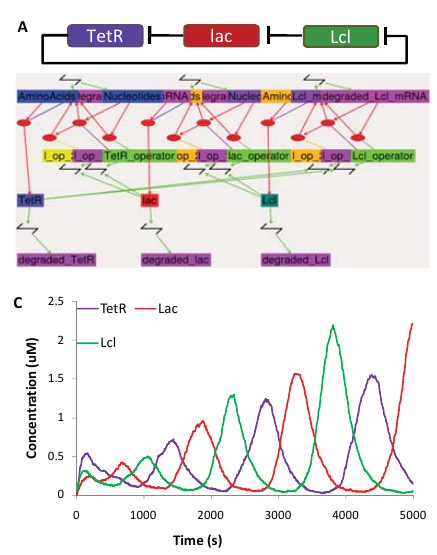
\includegraphics[width=0.55\textwidth]{./_images/reaction_diffusion_system.png}
    };
    \node[ text width = 0.48\textwidth] (reacdifft) at ([yshift=3cm]reacdiff.north) {
        \TEXT{
            Repressilator simulation based on Elowitz and Leibler (below).
            Enhanced reaction-diffusion capabilities in MOOSE (on right).
        }
    };
\end{tikzpicture}%  
\begin{tikzpicture} 
    \node[] (panelc) {
        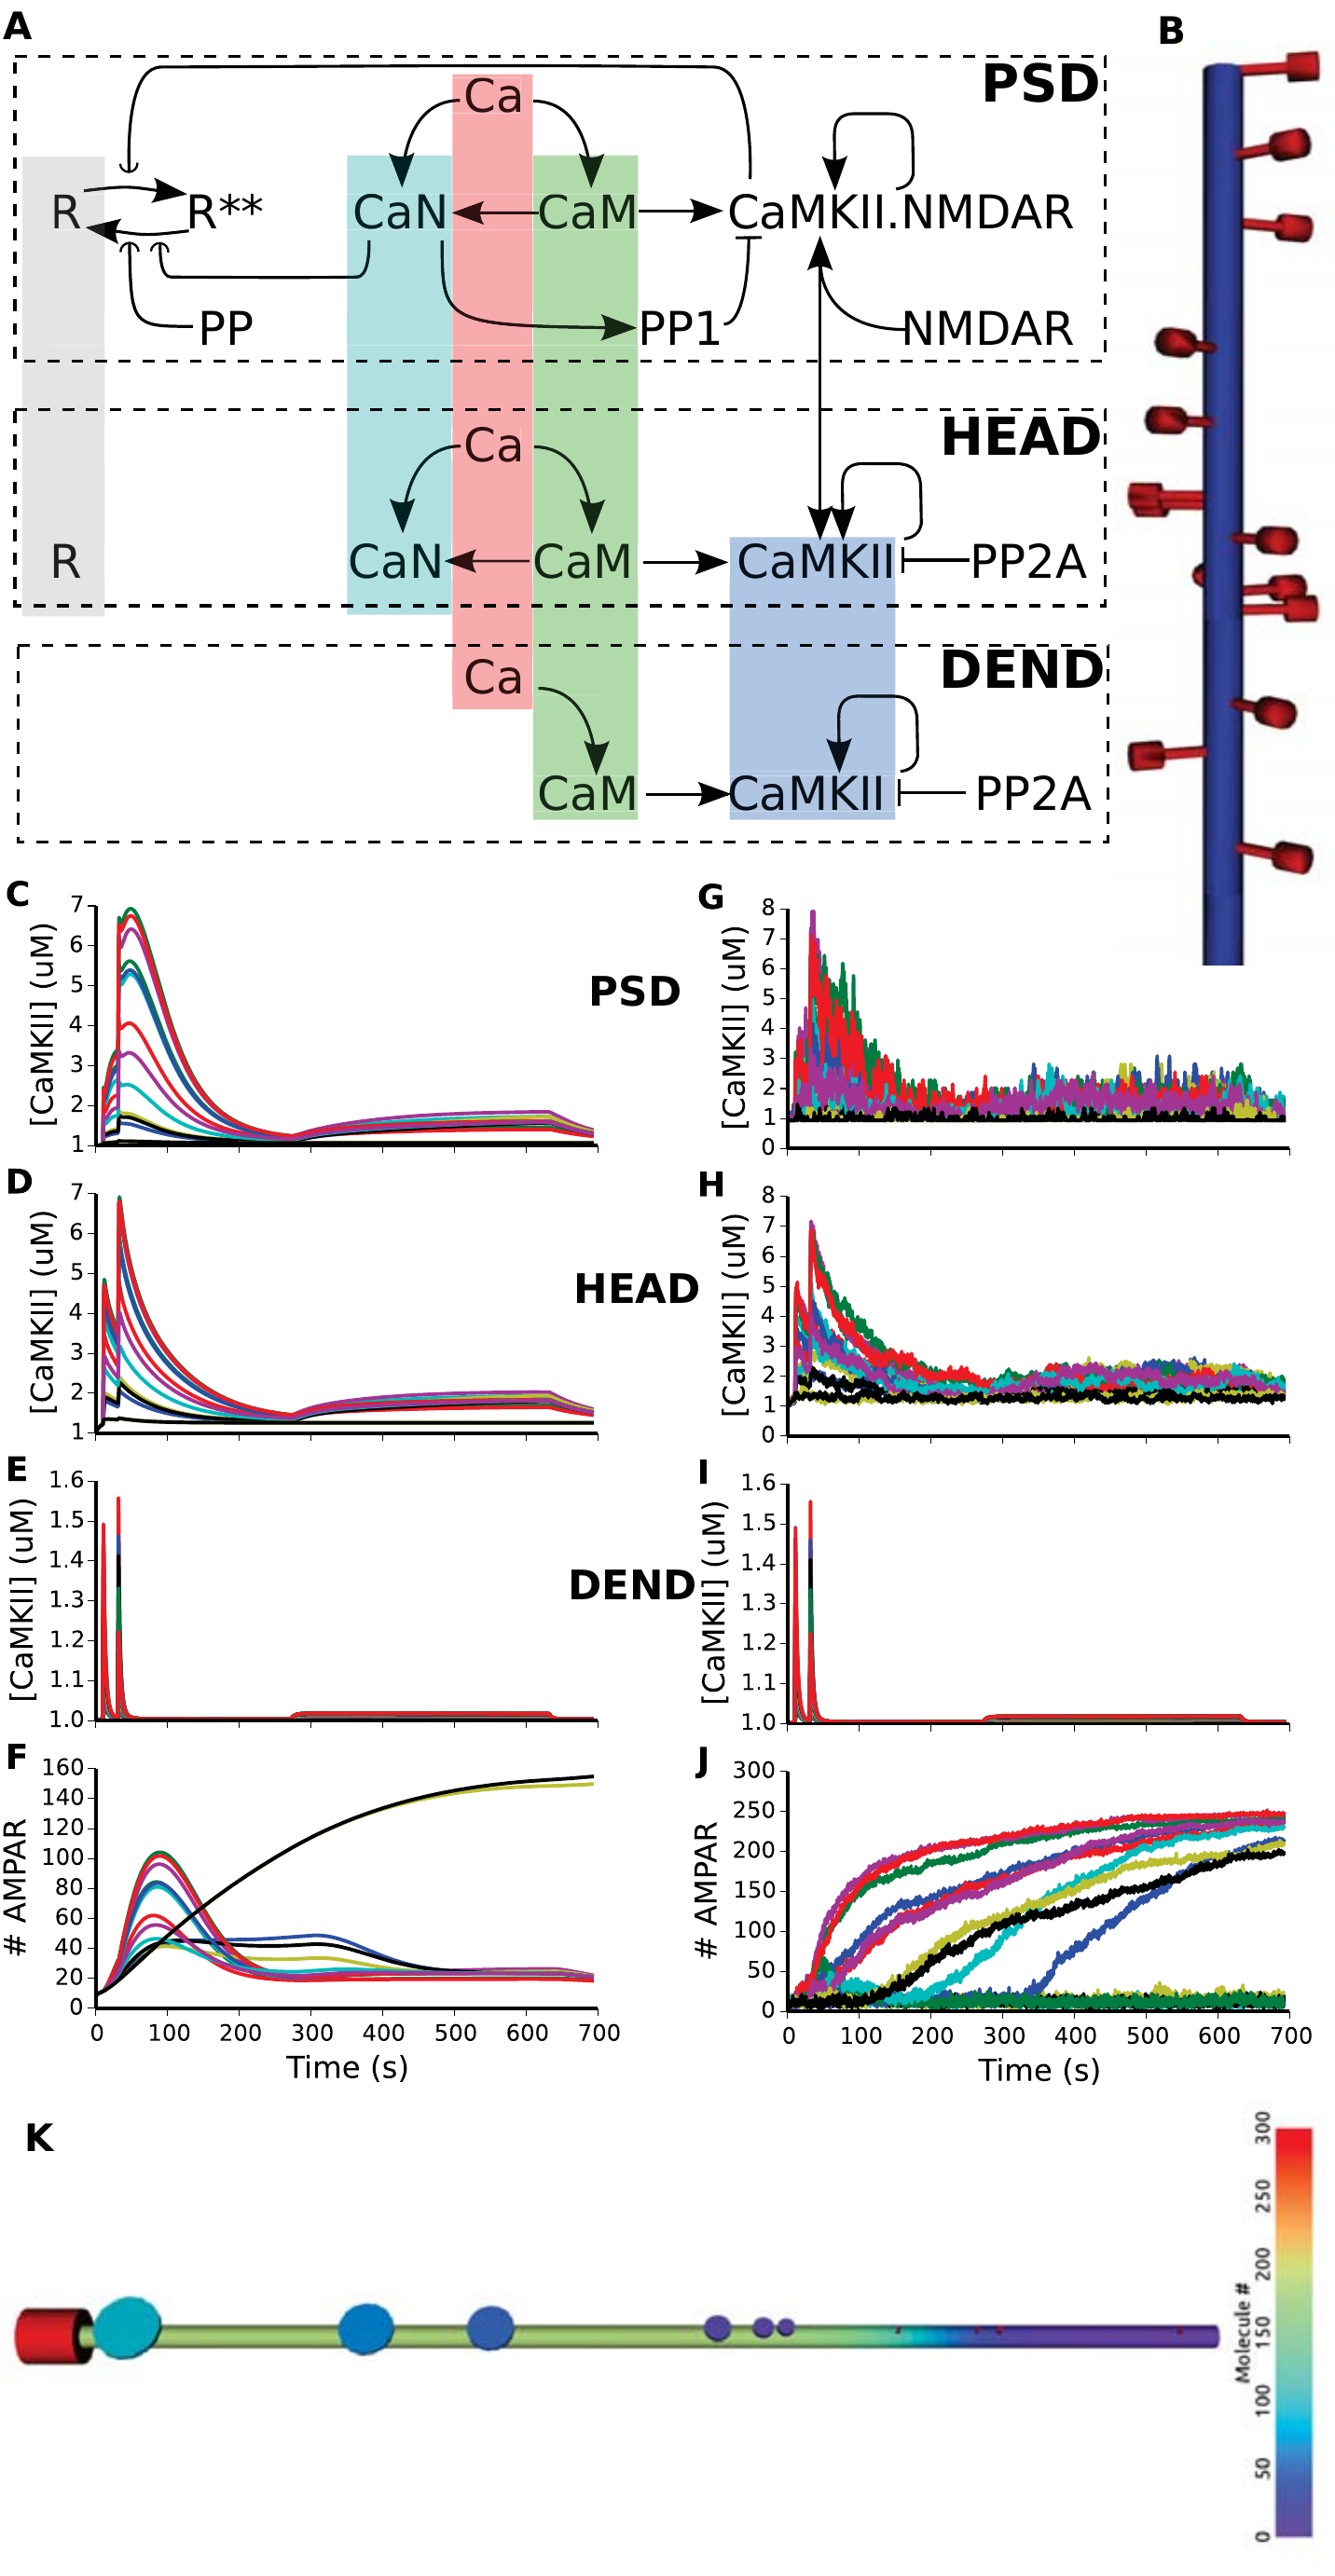
\includegraphics[width=0.4\textwidth]{./_images/panelc.png}
    };
    \node[text width=0.4\textwidth ] (panelct) at ([yshift=-3cm]panelc.south) {
        \TEXT{
            Three-comparment reaction scheme for CaMKII activation, translocation
            and receptor trafficking.
        }};

\end{tikzpicture} 

\vspace{1cm}
\HEADING{Modeling Memory}
\begin{tikzpicture}
    \node[ ] (paneld)  {
        \includegraphics[width=0.48\textwidth]{./_images/paneld.png}
    };
    \node[text width=0.48\textwidth] (paneldt) at ([yshift=2cm]paneld.north) {
        \TEXT{
            Molecule-to-network model. A detailed neuron embedded in network of
            2500 simple neurons with 20\% inhibitory neurons. 
        }
    };
\end{tikzpicture} %
\begin{tikzpicture}
    \node[ ] (chem) at ([yshift=2cm]0,0) {
        \includegraphics[width=0.48\textwidth]{./_images/chemical_computation.png}
    };
    \node[text width=0.48\textwidth] (chemt) at ([yshift=-3cm]chem.south) {
        \TEXT{
            Multiscale model in 4-different cell morphologies. Note the
            diversity of receptor insertion outcome!
        }
    };

\end{tikzpicture}


\end{Figure}

